\begin{figure}[!t]
\centering
\subfloat[]{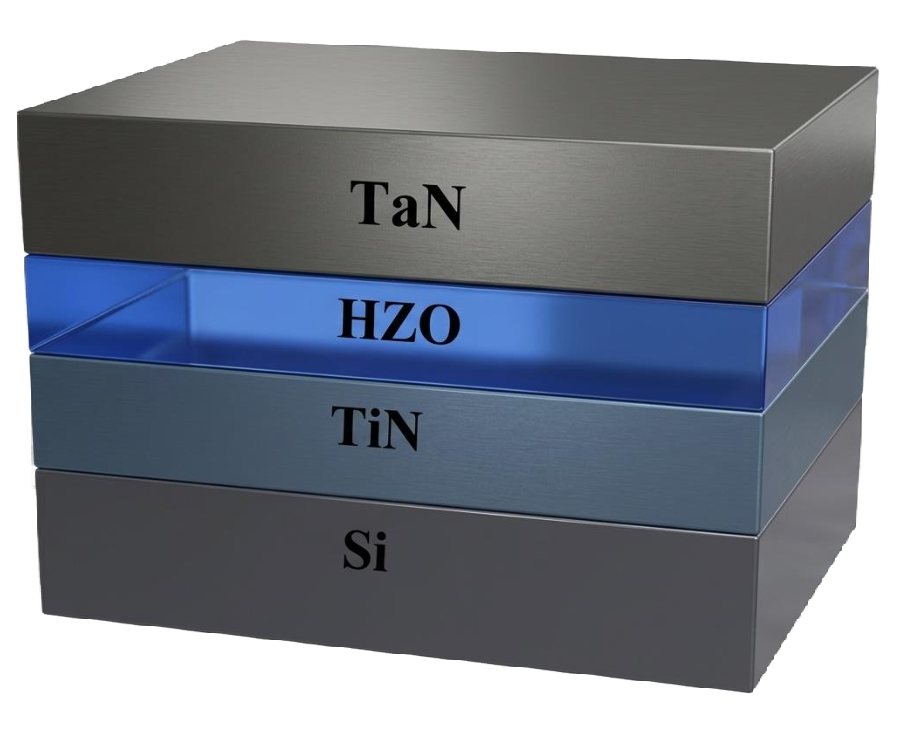
\includegraphics[width=0.47\columnwidth]{figures/fig 1a.pdf}\label{fig:stacks_a}}
\hfill
\subfloat[]{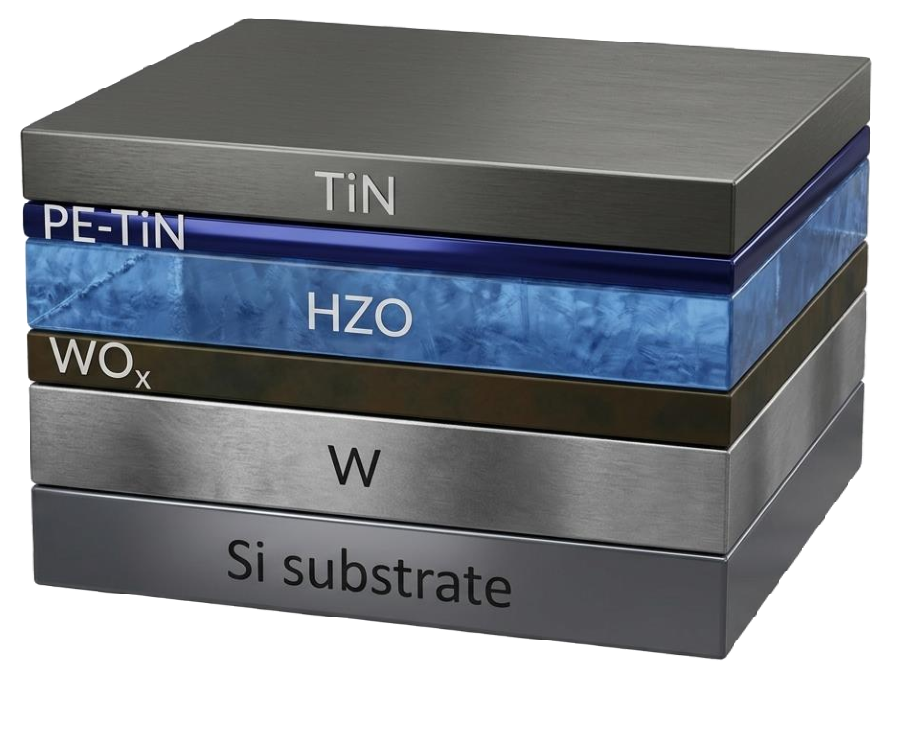
\includegraphics[width=0.47\columnwidth]{figures/fig 1b.pdf}\label{fig:stacks_b}}\\
\subfloat[]{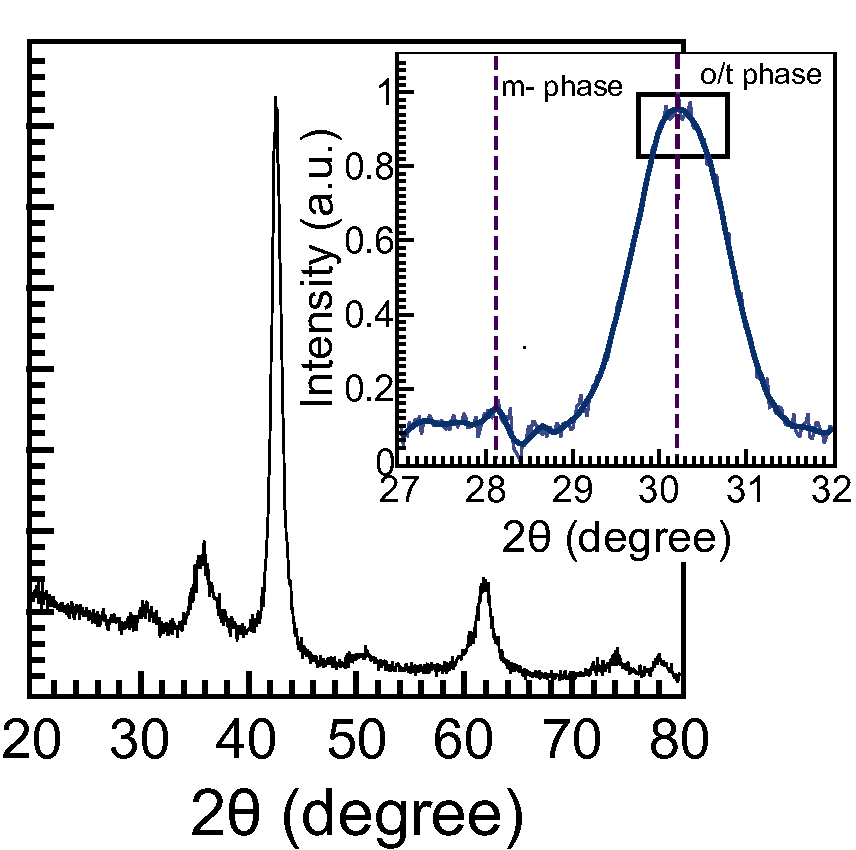
\includegraphics[width=0.47\columnwidth]{figures/1f_XRD Full.pdf}\label{fig:stacks_c}}
\hfill
\subfloat[]{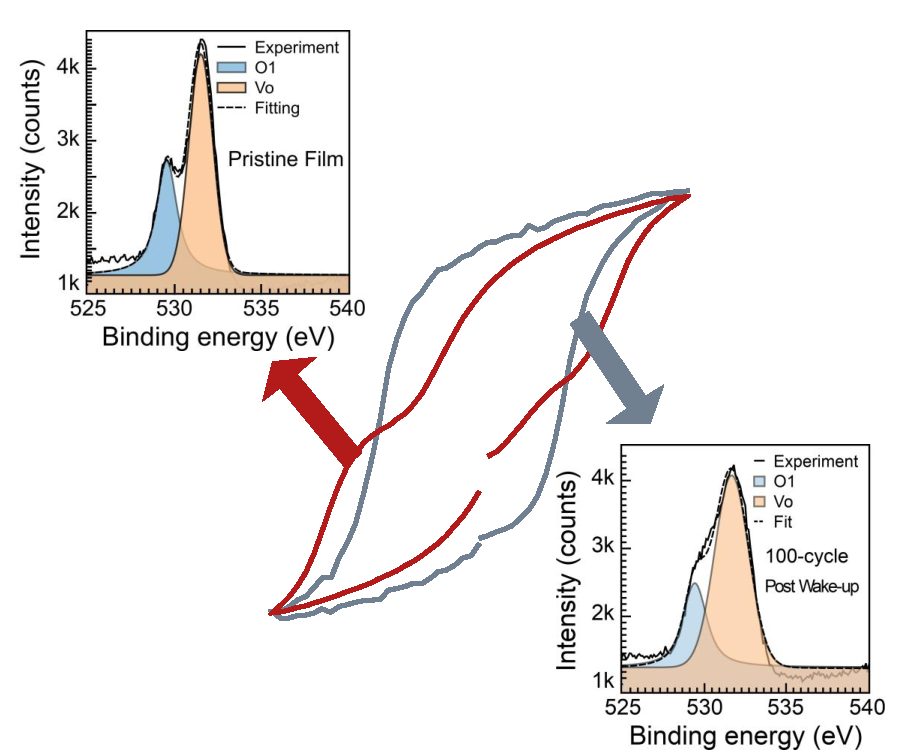
\includegraphics[width=0.47\columnwidth]{figures/fig 1d.pdf}\label{fig:stacks_d}}
\caption{Device and materials context. (a), (b) The compared capacitor stacks differ mainly in their electrode/interface design. (c) GIXRD confirms ferroelectric-phase formation in the \hzo{} films. (d) Polarization and interfacial-chemistry context from the source manuscript motivate the interface-focused interpretation used in this four-page version.}
\label{fig:stacks}
\end{figure}

\begin{figure}[!t]
\centering
\subfloat[]{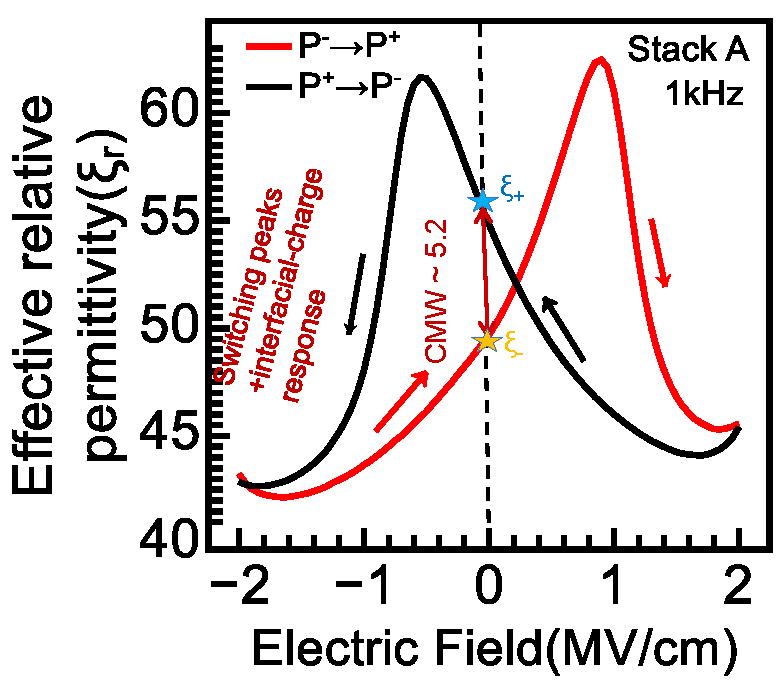
\includegraphics[width=0.47\columnwidth]{figures/fig 2a.pdf}\label{fig:cmw_a}}
\hfill
\subfloat[]{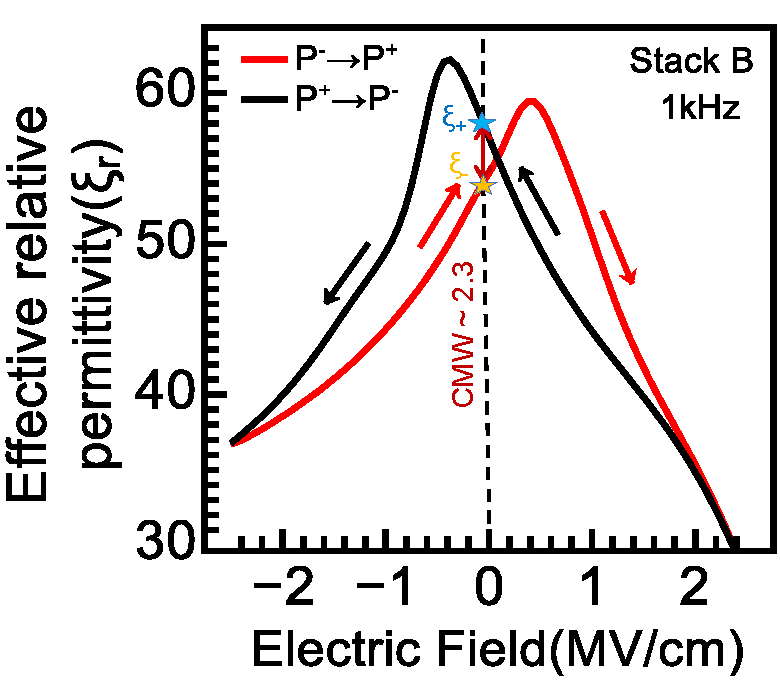
\includegraphics[width=0.47\columnwidth]{figures/fig 2b.pdf}\label{fig:cmw_b}}\\
\subfloat[]{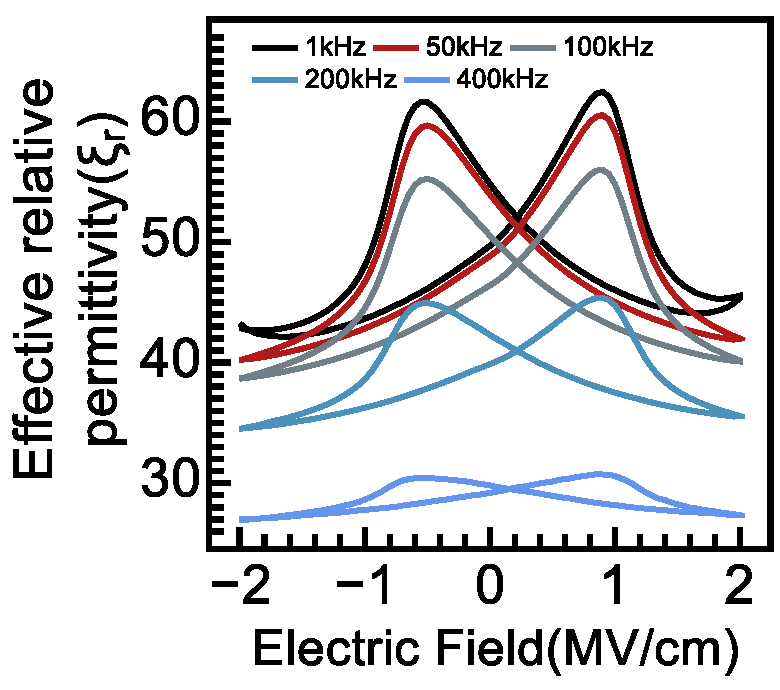
\includegraphics[width=0.47\columnwidth]{figures/fig 2c.pdf}\label{fig:cmw_c}}
\hfill
\subfloat[]{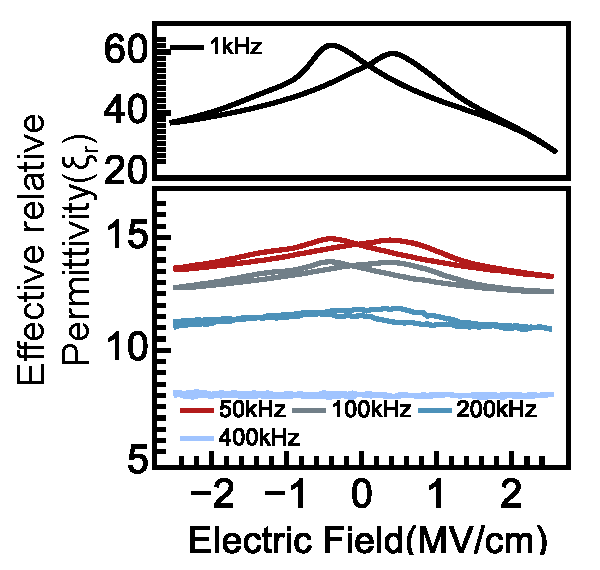
\includegraphics[width=0.47\columnwidth]{figures/fig 2d.pdf}\label{fig:cmw_d}}
\caption{Definition and collapse of the zero-bias CMW. Stack~A shows $\CMW_\xi \approx 5.2$ at 1~kHz, while Stack~B shows $\approx 2.3$ at a similar peak permittivity. With increasing frequency, the branch separation collapses while a substantial dielectric response remains, showing that the lost quantity is the state discrimination rather than the full capacitance.}
\label{fig:cmw}
\end{figure}

\begin{figure}[!t]
\centering
\subfloat[]{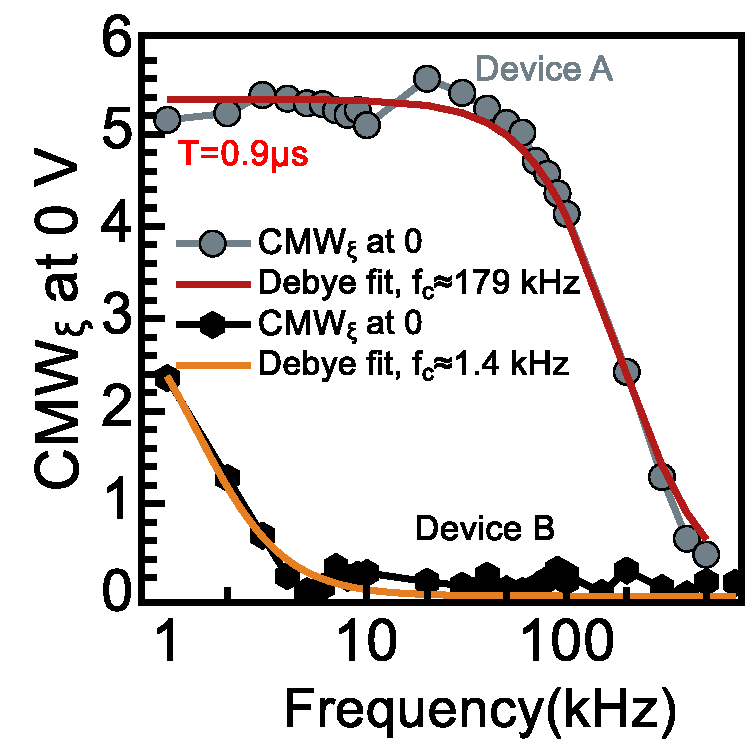
\includegraphics[width=0.31\columnwidth]{figures/fig 3a.pdf}\label{fig:debye_a}}
\hfill
\subfloat[]{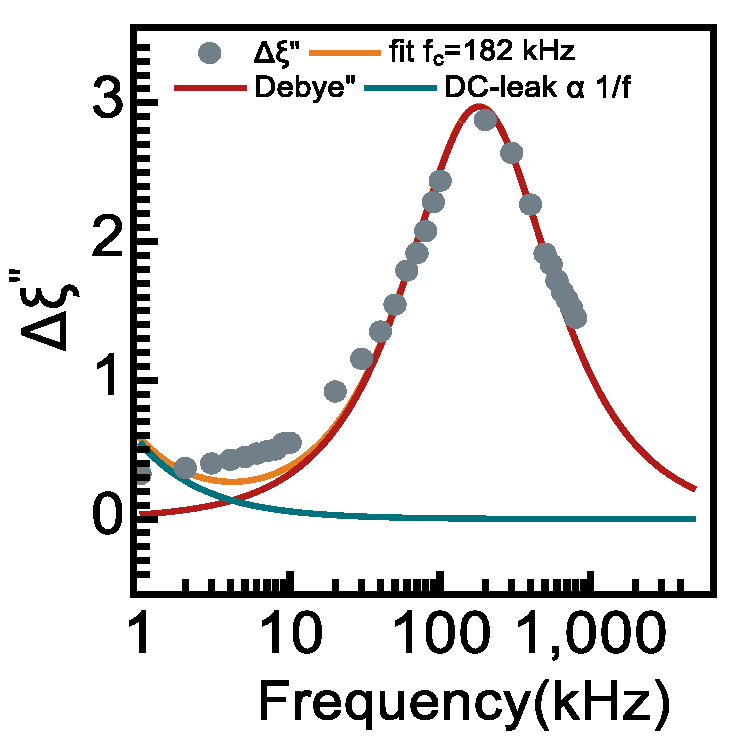
\includegraphics[width=0.31\columnwidth]{figures/fig 3b.pdf}\label{fig:debye_b}}
\hfill
\subfloat[]{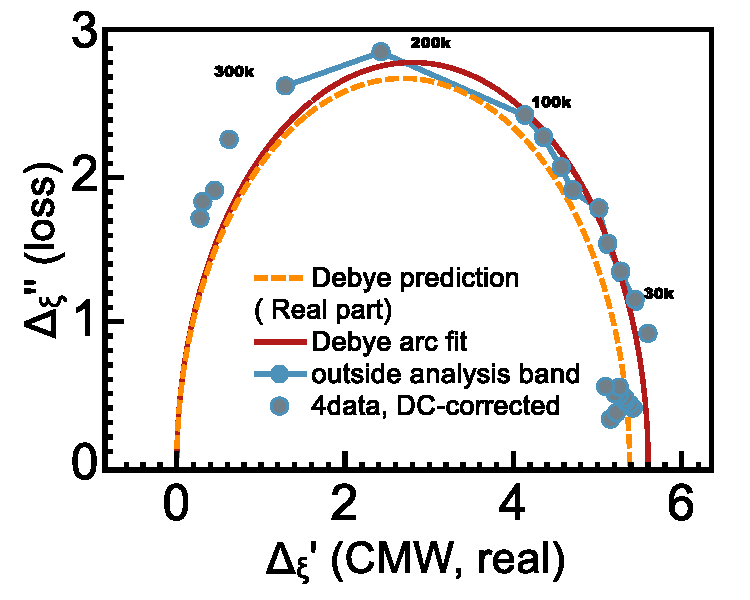
\includegraphics[width=0.31\columnwidth]{figures/fig 3c.pdf}\label{fig:debye_c}}
\caption{Single-process relaxation evidence. The CMW roll-off, differential loss, and Cole--Cole response are all consistent with a single-Debye relaxation, giving $\fc=179$~kHz for Stack~A and $\fc=1.4$~kHz for Stack~B.}
\label{fig:debye}
\end{figure}

\begin{figure}[!t]
\centering
\subfloat[]{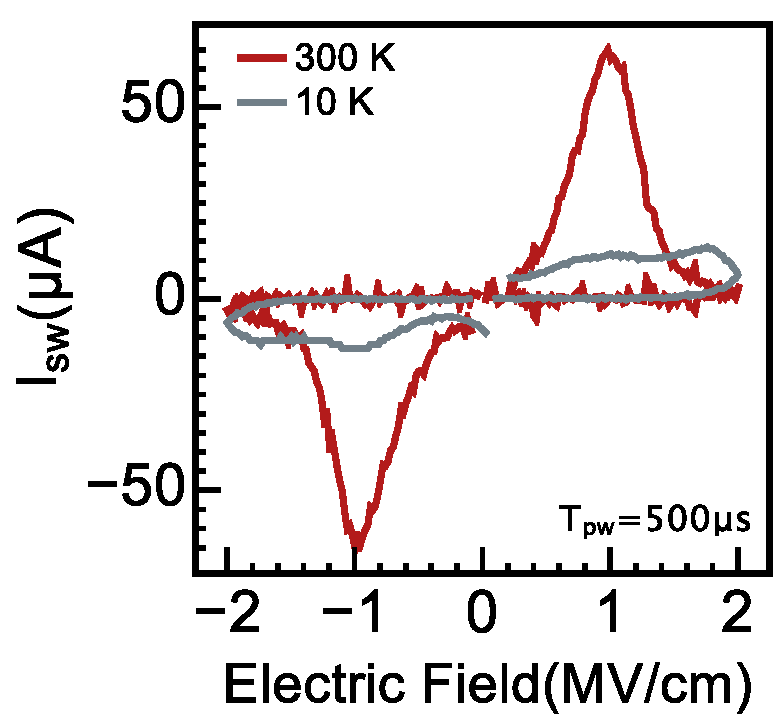
\includegraphics[width=0.47\columnwidth]{figures/fig 4a.pdf}\label{fig:cryo_a}}
\hfill
\subfloat[]{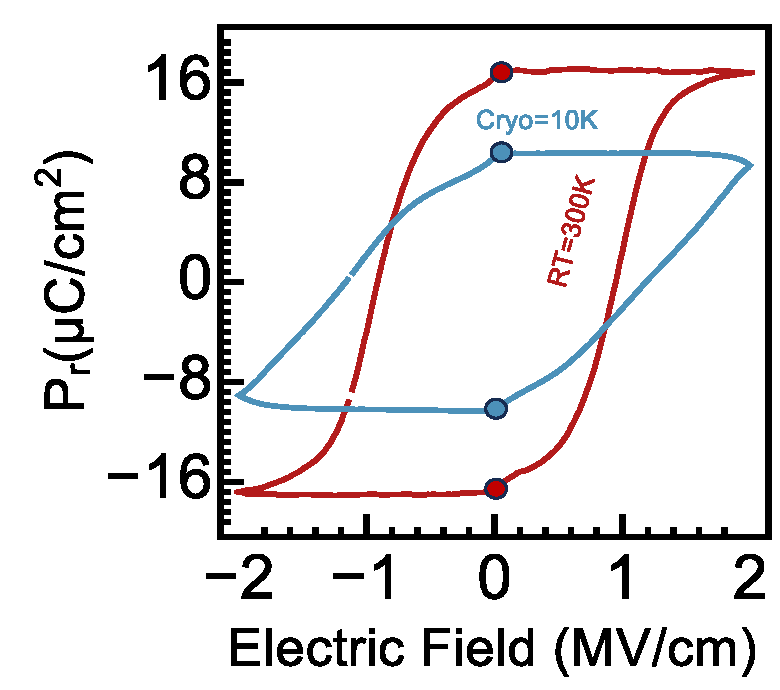
\includegraphics[width=0.47\columnwidth]{figures/fig 5b.pdf}\label{fig:cryo_b}}\\
\subfloat[]{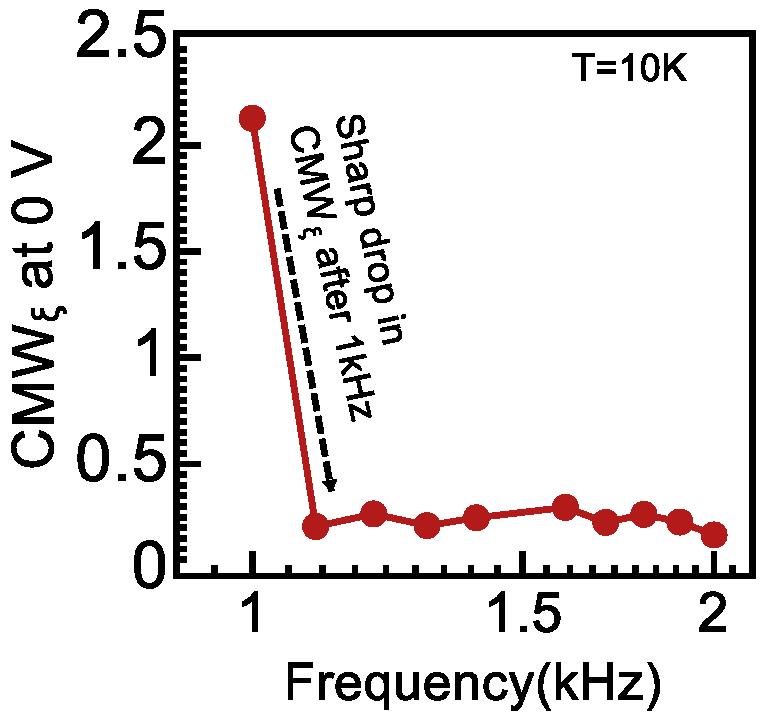
\includegraphics[width=0.47\columnwidth]{figures/fig 4d.pdf}\label{fig:cryo_c}}
\hfill
\subfloat[]{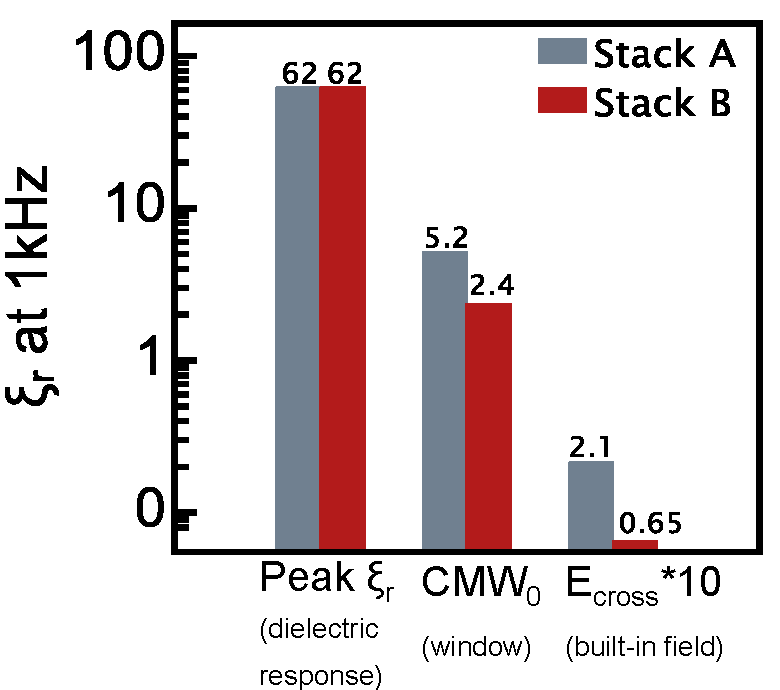
\includegraphics[width=0.47\columnwidth]{figures/figure3/fig 3e.pdf}\label{fig:cryo_d}}
\caption{Temperature and interface summary. At 10~K, switching persists but the zero-bias CMW bandwidth collapses below 1~kHz. The cross-stack summary shows nearly identical low-frequency dielectric ceilings together with large differences in CMW amplitude and clock speed, consistent with interface-controlled readout.}
\label{fig:cryo}
\end{figure}

\begin{table}[!t]
\renewcommand{\arraystretch}{1.08}
\caption{Key Parameters Retained for the 4-Page Version}
\label{tab:summary}
\centering
\scriptsize
\setlength{\tabcolsep}{3pt}
\begin{tabular}{@{}lcc@{}}
\toprule
Parameter & Stack A & Stack B \\
\midrule
Peak $\xir$ at 1 kHz & 62.5 & 62.2 \\
Ceiling $\xir(0)$ & $62.4\pm1.2$ & $62.7\pm0.9$ \\
CMW at 1 kHz & 5.2 & 2.4 \\
$\CMW_0$ (fit) & 5.38 & 3.6 \\
$\fc$ & 179 kHz & 1.4 kHz \\
$\tau$ & 0.90 $\mu$s & 114 $\mu$s \\
$\Ecross$ & 0.221 MV/cm & 0.081 MV/cm \\
$c_{IL}$ & 2.95 $\mu$F/cm$^2$ & 2.34 $\mu$F/cm$^2$ \\
$R_{IL}$ & 0.31 $\Omega\cdot$cm$^2$ & 48.8 $\Omega\cdot$cm$^2$ \\
\midrule
$2P_r$ at 300 K / 10 K & \multicolumn{2}{c}{33.1 / 20.3 $\mu$C/cm$^2$} \\
CMW at 300 K / 10 K & \multicolumn{2}{c}{5.2 / 2.2 (Stack~A)} \\
$\fc$ at 300 K / 10 K & \multicolumn{2}{c}{179 kHz / $\lesssim$1 kHz (Stack~A)} \\
\bottomrule
\end{tabular}
\end{table}
